\documentclass[twoside]{book}

% Packages required by doxygen
\usepackage{fixltx2e}
\usepackage{calc}
\usepackage{doxygen}
\usepackage[export]{adjustbox} % also loads graphicx
\usepackage{graphicx}
\usepackage[utf8]{inputenc}
\usepackage{makeidx}
\usepackage{multicol}
\usepackage{multirow}
\PassOptionsToPackage{warn}{textcomp}
\usepackage{textcomp}
\usepackage[nointegrals]{wasysym}
\usepackage[table]{xcolor}

% Font selection
\usepackage[T1]{fontenc}
\usepackage[scaled=.90]{helvet}
\usepackage{courier}
\usepackage{amssymb}
\usepackage{sectsty}
\renewcommand{\familydefault}{\sfdefault}
\allsectionsfont{%
  \fontseries{bc}\selectfont%
  \color{darkgray}%
}
\renewcommand{\DoxyLabelFont}{%
  \fontseries{bc}\selectfont%
  \color{darkgray}%
}
\newcommand{\+}{\discretionary{\mbox{\scriptsize$\hookleftarrow$}}{}{}}

% Page & text layout
\usepackage{geometry}
\geometry{%
  a4paper,%
  top=2.5cm,%
  bottom=2.5cm,%
  left=2.5cm,%
  right=2.5cm%
}
\tolerance=750
\hfuzz=15pt
\hbadness=750
\setlength{\emergencystretch}{15pt}
\setlength{\parindent}{0cm}
\setlength{\parskip}{3ex plus 2ex minus 2ex}
\makeatletter
\renewcommand{\paragraph}{%
  \@startsection{paragraph}{4}{0ex}{-1.0ex}{1.0ex}{%
    \normalfont\normalsize\bfseries\SS@parafont%
  }%
}
\renewcommand{\subparagraph}{%
  \@startsection{subparagraph}{5}{0ex}{-1.0ex}{1.0ex}{%
    \normalfont\normalsize\bfseries\SS@subparafont%
  }%
}
\makeatother

% Headers & footers
\usepackage{fancyhdr}
\pagestyle{fancyplain}
\fancyhead[LE]{\fancyplain{}{\bfseries\thepage}}
\fancyhead[CE]{\fancyplain{}{}}
\fancyhead[RE]{\fancyplain{}{\bfseries\leftmark}}
\fancyhead[LO]{\fancyplain{}{\bfseries\rightmark}}
\fancyhead[CO]{\fancyplain{}{}}
\fancyhead[RO]{\fancyplain{}{\bfseries\thepage}}
\fancyfoot[LE]{\fancyplain{}{}}
\fancyfoot[CE]{\fancyplain{}{}}
\fancyfoot[RE]{\fancyplain{}{\bfseries\scriptsize Generated by Doxygen }}
\fancyfoot[LO]{\fancyplain{}{\bfseries\scriptsize Generated by Doxygen }}
\fancyfoot[CO]{\fancyplain{}{}}
\fancyfoot[RO]{\fancyplain{}{}}
\renewcommand{\footrulewidth}{0.4pt}
\renewcommand{\chaptermark}[1]{%
  \markboth{#1}{}%
}
\renewcommand{\sectionmark}[1]{%
  \markright{\thesection\ #1}%
}

% Indices & bibliography
\usepackage{natbib}
\usepackage[titles]{tocloft}
\setcounter{tocdepth}{3}
\setcounter{secnumdepth}{5}
\makeindex

% Hyperlinks (required, but should be loaded last)
\usepackage{ifpdf}
\ifpdf
  \usepackage[pdftex,pagebackref=true]{hyperref}
\else
  \usepackage[ps2pdf,pagebackref=true]{hyperref}
\fi
\hypersetup{%
  colorlinks=true,%
  linkcolor=blue,%
  citecolor=blue,%
  unicode%
}

% Custom commands
\newcommand{\clearemptydoublepage}{%
  \newpage{\pagestyle{empty}\cleardoublepage}%
}

\usepackage{caption}
\captionsetup{labelsep=space,justification=centering,font={bf},singlelinecheck=off,skip=4pt,position=top}

%===== C O N T E N T S =====

\begin{document}

% Titlepage & ToC
\hypersetup{pageanchor=false,
             bookmarksnumbered=true,
             pdfencoding=unicode
            }
\pagenumbering{alph}
\begin{titlepage}
\vspace*{7cm}
\begin{center}%
{\Large My Project }\\
\vspace*{1cm}
{\large Generated by Doxygen 1.8.13}\\
\end{center}
\end{titlepage}
\clearemptydoublepage
\pagenumbering{roman}
\tableofcontents
\clearemptydoublepage
\pagenumbering{arabic}
\hypersetup{pageanchor=true}

%--- Begin generated contents ---
\chapter{Hierarchical Index}
\section{Class Hierarchy}
This inheritance list is sorted roughly, but not completely, alphabetically\+:\begin{DoxyCompactList}
\item \contentsline{section}{Figura\+Geometrica}{\pageref{class_figura_geometrica}}{}
\begin{DoxyCompactList}
\item \contentsline{section}{Circulo}{\pageref{class_circulo}}{}
\item \contentsline{section}{Reta}{\pageref{class_reta}}{}
\item \contentsline{section}{Retangulo}{\pageref{class_retangulo}}{}
\end{DoxyCompactList}
\item \contentsline{section}{Screen}{\pageref{class_screen}}{}
\end{DoxyCompactList}

\chapter{Class Index}
\section{Class List}
Here are the classes, structs, unions and interfaces with brief descriptions\+:\begin{DoxyCompactList}
\item\contentsline{section}{\hyperlink{class_circulo}{Circulo} \\*É uma classe concreta derivada d classe \hyperlink{class_figura_geometrica}{Figura\+Geometrica} que cria um círculo }{\pageref{class_circulo}}{}
\item\contentsline{section}{\hyperlink{class_figura_geometrica}{Figura\+Geometrica} \\*É uma classe abastrada utilizada para desenvolver figuras geométricas }{\pageref{class_figura_geometrica}}{}
\item\contentsline{section}{\hyperlink{class_reta}{Reta} \\*É uma classe concreta derivada d classe \hyperlink{class_figura_geometrica}{Figura\+Geometrica} que cria uma reta }{\pageref{class_reta}}{}
\item\contentsline{section}{\hyperlink{class_retangulo}{Retangulo} \\*É uma classe concreta derivada d classe \hyperlink{class_figura_geometrica}{Figura\+Geometrica} que cria um retângulo }{\pageref{class_retangulo}}{}
\item\contentsline{section}{\hyperlink{class_screen}{Screen} \\*Funciona criando e editando telas de desenho }{\pageref{class_screen}}{}
\end{DoxyCompactList}

\chapter{Class Documentation}
\hypertarget{class_circulo}{}\section{Circulo Class Reference}
\label{class_circulo}\index{Circulo@{Circulo}}


The \hyperlink{class_circulo}{Circulo} class É uma classe concreta derivada d classe \hyperlink{class_figura_geometrica}{Figura\+Geometrica} que cria um círculo.  




{\ttfamily \#include $<$circulo.\+h$>$}



Inheritance diagram for Circulo\+:
\nopagebreak
\begin{figure}[H]
\begin{center}
\leavevmode
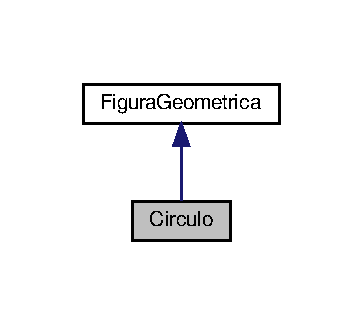
\includegraphics[width=174pt]{class_circulo__inherit__graph}
\end{center}
\end{figure}


Collaboration diagram for Circulo\+:
\nopagebreak
\begin{figure}[H]
\begin{center}
\leavevmode
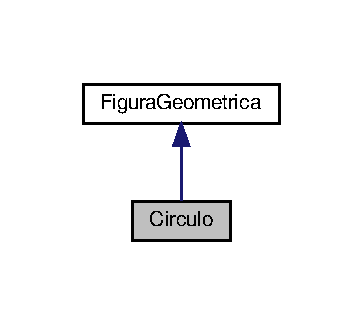
\includegraphics[width=174pt]{class_circulo__coll__graph}
\end{center}
\end{figure}
\subsection*{Public Member Functions}
\begin{DoxyCompactItemize}
\item 
\hyperlink{class_circulo_a25ea8ad5025f200c8459e81048bd34c5}{Circulo} (int x0\+\_\+, int y0\+\_\+, int r\+\_\+, bool fill\+\_\+=false)
\begin{DoxyCompactList}\small\item\em \hyperlink{class_circulo}{Circulo} Cria um círculo a partir do seu centro cum um determinado raio. \end{DoxyCompactList}\item 
void \hyperlink{class_circulo_a593787d6e0618c2eded23e8839e7bea6}{draw} (\hyperlink{class_screen}{Screen} \&t)
\begin{DoxyCompactList}\small\item\em draw Método virtual que força ponteiros para apontar a suas derivadas; \end{DoxyCompactList}\end{DoxyCompactItemize}


\subsection{Detailed Description}
The \hyperlink{class_circulo}{Circulo} class É uma classe concreta derivada d classe \hyperlink{class_figura_geometrica}{Figura\+Geometrica} que cria um círculo. 

\subsection{Constructor \& Destructor Documentation}
\mbox{\Hypertarget{class_circulo_a25ea8ad5025f200c8459e81048bd34c5}\label{class_circulo_a25ea8ad5025f200c8459e81048bd34c5}} 
\index{Circulo@{Circulo}!Circulo@{Circulo}}
\index{Circulo@{Circulo}!Circulo@{Circulo}}
\subsubsection{\texorpdfstring{Circulo()}{Circulo()}}
{\footnotesize\ttfamily Circulo\+::\+Circulo (\begin{DoxyParamCaption}\item[{int}]{x0\+\_\+,  }\item[{int}]{y0\+\_\+,  }\item[{int}]{r\+\_\+,  }\item[{bool}]{fill\+\_\+ = {\ttfamily false} }\end{DoxyParamCaption})}



\hyperlink{class_circulo}{Circulo} Cria um círculo a partir do seu centro cum um determinado raio. 


\begin{DoxyParams}{Parameters}
{\em x0\+\_\+} & É a coordenada x do centro do círculo. \\
\hline
{\em y0\+\_\+} & É a coordenada y do centro do círculo. \\
\hline
{\em r\+\_\+} & É o raio do círculo. \\
\hline
{\em fill\+\_\+} & Determina se o cículo será preenchido (true) ou não (false) \\
\hline
\end{DoxyParams}


\subsection{Member Function Documentation}
\mbox{\Hypertarget{class_circulo_a593787d6e0618c2eded23e8839e7bea6}\label{class_circulo_a593787d6e0618c2eded23e8839e7bea6}} 
\index{Circulo@{Circulo}!draw@{draw}}
\index{draw@{draw}!Circulo@{Circulo}}
\subsubsection{\texorpdfstring{draw()}{draw()}}
{\footnotesize\ttfamily void Circulo\+::draw (\begin{DoxyParamCaption}\item[{\hyperlink{class_screen}{Screen} \&}]{t }\end{DoxyParamCaption})\hspace{0.3cm}{\ttfamily [virtual]}}



draw Método virtual que força ponteiros para apontar a suas derivadas; 


\begin{DoxyParams}{Parameters}
{\em t} & Tela em que as figuras serão desenhadas. \\
\hline
\end{DoxyParams}


Implements \hyperlink{class_figura_geometrica_a8ee8dedc060b6059a805ea091aef2c41}{Figura\+Geometrica}.



The documentation for this class was generated from the following files\+:\begin{DoxyCompactItemize}
\item 
circulo.\+h\item 
circulo.\+cpp\end{DoxyCompactItemize}

\hypertarget{class_figura_geometrica}{}\section{Figura\+Geometrica Class Reference}
\label{class_figura_geometrica}\index{Figura\+Geometrica@{Figura\+Geometrica}}


The \hyperlink{class_figura_geometrica}{Figura\+Geometrica} class É uma classe abastrada utilizada para desenvolver figuras geométricas.  




{\ttfamily \#include $<$figurageometrica.\+h$>$}



Inheritance diagram for Figura\+Geometrica\+:
\nopagebreak
\begin{figure}[H]
\begin{center}
\leavevmode
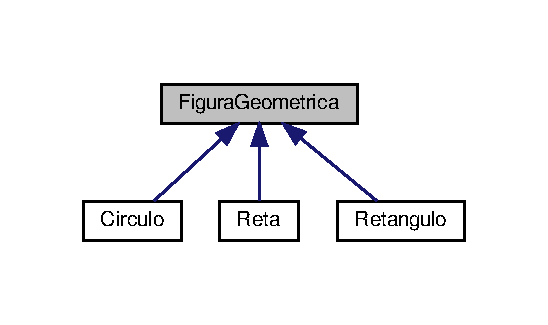
\includegraphics[width=263pt]{class_figura_geometrica__inherit__graph}
\end{center}
\end{figure}
\subsection*{Public Member Functions}
\begin{DoxyCompactItemize}
\item 
\mbox{\Hypertarget{class_figura_geometrica_a81d7c7efaea511e60a15f5a363138dd9}\label{class_figura_geometrica_a81d7c7efaea511e60a15f5a363138dd9}} 
\hyperlink{class_figura_geometrica_a81d7c7efaea511e60a15f5a363138dd9}{Figura\+Geometrica} ()
\begin{DoxyCompactList}\small\item\em \hyperlink{class_figura_geometrica}{Figura\+Geometrica} É o construtor padrão da classe. \end{DoxyCompactList}\item 
virtual void \hyperlink{class_figura_geometrica_a8ee8dedc060b6059a805ea091aef2c41}{draw} (\hyperlink{class_screen}{Screen} \&t)=0
\begin{DoxyCompactList}\small\item\em draw Método virtual que força ponteiros para apontar a suas derivadas; \end{DoxyCompactList}\end{DoxyCompactItemize}


\subsection{Detailed Description}
The \hyperlink{class_figura_geometrica}{Figura\+Geometrica} class É uma classe abastrada utilizada para desenvolver figuras geométricas. 

\subsection{Member Function Documentation}
\mbox{\Hypertarget{class_figura_geometrica_a8ee8dedc060b6059a805ea091aef2c41}\label{class_figura_geometrica_a8ee8dedc060b6059a805ea091aef2c41}} 
\index{Figura\+Geometrica@{Figura\+Geometrica}!draw@{draw}}
\index{draw@{draw}!Figura\+Geometrica@{Figura\+Geometrica}}
\subsubsection{\texorpdfstring{draw()}{draw()}}
{\footnotesize\ttfamily virtual void Figura\+Geometrica\+::draw (\begin{DoxyParamCaption}\item[{\hyperlink{class_screen}{Screen} \&}]{t }\end{DoxyParamCaption})\hspace{0.3cm}{\ttfamily [pure virtual]}}



draw Método virtual que força ponteiros para apontar a suas derivadas; 


\begin{DoxyParams}{Parameters}
{\em t} & Tela em que as figuras serão desenhadas. \\
\hline
\end{DoxyParams}


Implemented in \hyperlink{class_retangulo_ac088dd6d3f4f3d3f80363a868c2e74f1}{Retangulo}, \hyperlink{class_reta_ac2e9805183cd474b62bffd8b032cd780}{Reta}, and \hyperlink{class_circulo_a593787d6e0618c2eded23e8839e7bea6}{Circulo}.



The documentation for this class was generated from the following files\+:\begin{DoxyCompactItemize}
\item 
figurageometrica.\+h\item 
figurageometrica.\+cpp\end{DoxyCompactItemize}

\hypertarget{class_reta}{}\section{Reta Class Reference}
\label{class_reta}\index{Reta@{Reta}}


The \hyperlink{class_reta}{Reta} class É uma classe concreta derivada d classe \hyperlink{class_figura_geometrica}{Figura\+Geometrica} que cria uma reta.  




{\ttfamily \#include $<$reta.\+h$>$}



Inheritance diagram for Reta\+:
\nopagebreak
\begin{figure}[H]
\begin{center}
\leavevmode
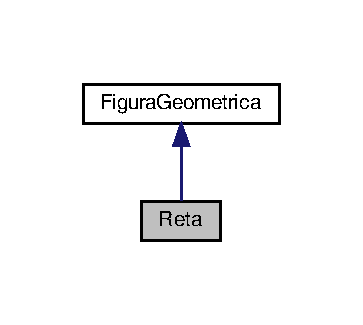
\includegraphics[width=174pt]{class_reta__inherit__graph}
\end{center}
\end{figure}


Collaboration diagram for Reta\+:
\nopagebreak
\begin{figure}[H]
\begin{center}
\leavevmode
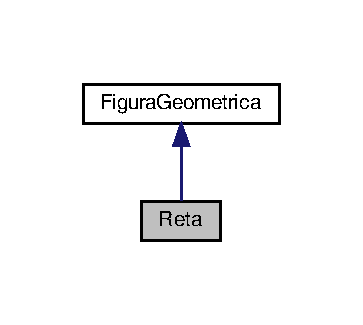
\includegraphics[width=174pt]{class_reta__coll__graph}
\end{center}
\end{figure}
\subsection*{Public Member Functions}
\begin{DoxyCompactItemize}
\item 
\hyperlink{class_reta_a9e125389d2176bba3c1430f5041beb83}{Reta} (int x1\+\_\+, int y1\+\_\+, int x2\+\_\+, int y2\+\_\+)
\begin{DoxyCompactList}\small\item\em \hyperlink{class_reta}{Reta} Cria um reta que vai do ponto (x1,y1) até o ponto (x2,y2) \end{DoxyCompactList}\item 
void \hyperlink{class_reta_ac2e9805183cd474b62bffd8b032cd780}{draw} (\hyperlink{class_screen}{Screen} \&t)
\begin{DoxyCompactList}\small\item\em draw Desenha uma reta na tela t. \end{DoxyCompactList}\item 
int \hyperlink{class_reta_ac148699b1fd8a77732d9e0546318ad58}{Sinal} (float n)
\begin{DoxyCompactList}\small\item\em Sinal Analisa o sinal de um número em ponto flutuante. \end{DoxyCompactList}\end{DoxyCompactItemize}


\subsection{Detailed Description}
The \hyperlink{class_reta}{Reta} class É uma classe concreta derivada d classe \hyperlink{class_figura_geometrica}{Figura\+Geometrica} que cria uma reta. 

\subsection{Constructor \& Destructor Documentation}
\mbox{\Hypertarget{class_reta_a9e125389d2176bba3c1430f5041beb83}\label{class_reta_a9e125389d2176bba3c1430f5041beb83}} 
\index{Reta@{Reta}!Reta@{Reta}}
\index{Reta@{Reta}!Reta@{Reta}}
\subsubsection{\texorpdfstring{Reta()}{Reta()}}
{\footnotesize\ttfamily Reta\+::\+Reta (\begin{DoxyParamCaption}\item[{int}]{x1\+\_\+,  }\item[{int}]{y1\+\_\+,  }\item[{int}]{x2\+\_\+,  }\item[{int}]{y2\+\_\+ }\end{DoxyParamCaption})}



\hyperlink{class_reta}{Reta} Cria um reta que vai do ponto (x1,y1) até o ponto (x2,y2) 


\begin{DoxyParams}{Parameters}
{\em x1\+\_\+} & Coordenada x do ponto 1 \\
\hline
{\em y1\+\_\+} & Coordenada y do ponto 1 \\
\hline
{\em x2\+\_\+} & Coordenada x do ponto 2 \\
\hline
{\em y2\+\_\+} & Coordenada y do ponto 2 \\
\hline
\end{DoxyParams}


\subsection{Member Function Documentation}
\mbox{\Hypertarget{class_reta_ac2e9805183cd474b62bffd8b032cd780}\label{class_reta_ac2e9805183cd474b62bffd8b032cd780}} 
\index{Reta@{Reta}!draw@{draw}}
\index{draw@{draw}!Reta@{Reta}}
\subsubsection{\texorpdfstring{draw()}{draw()}}
{\footnotesize\ttfamily void Reta\+::draw (\begin{DoxyParamCaption}\item[{\hyperlink{class_screen}{Screen} \&}]{t }\end{DoxyParamCaption})\hspace{0.3cm}{\ttfamily [virtual]}}



draw Desenha uma reta na tela t. 


\begin{DoxyParams}{Parameters}
{\em t} & Tela em que será desenhada a reta. \\
\hline
\end{DoxyParams}


Implements \hyperlink{class_figura_geometrica_a8ee8dedc060b6059a805ea091aef2c41}{Figura\+Geometrica}.

\mbox{\Hypertarget{class_reta_ac148699b1fd8a77732d9e0546318ad58}\label{class_reta_ac148699b1fd8a77732d9e0546318ad58}} 
\index{Reta@{Reta}!Sinal@{Sinal}}
\index{Sinal@{Sinal}!Reta@{Reta}}
\subsubsection{\texorpdfstring{Sinal()}{Sinal()}}
{\footnotesize\ttfamily int Reta\+::\+Sinal (\begin{DoxyParamCaption}\item[{float}]{n }\end{DoxyParamCaption})}



Sinal Analisa o sinal de um número em ponto flutuante. 


\begin{DoxyParams}{Parameters}
{\em n} & Número a ser analisado. \\
\hline
\end{DoxyParams}
\begin{DoxyReturn}{Returns}
1, se n for postivo; 0, se n=0; -\/1, se n for negativo 
\end{DoxyReturn}


The documentation for this class was generated from the following files\+:\begin{DoxyCompactItemize}
\item 
reta.\+h\item 
reta.\+cpp\end{DoxyCompactItemize}

\hypertarget{class_retangulo}{}\section{Retangulo Class Reference}
\label{class_retangulo}\index{Retangulo@{Retangulo}}


The \hyperlink{class_retangulo}{Retangulo} class É uma classe concreta derivada d classe \hyperlink{class_figura_geometrica}{Figura\+Geometrica} que cria um retângulo.  




{\ttfamily \#include $<$retangulo.\+h$>$}



Inheritance diagram for Retangulo\+:
\nopagebreak
\begin{figure}[H]
\begin{center}
\leavevmode
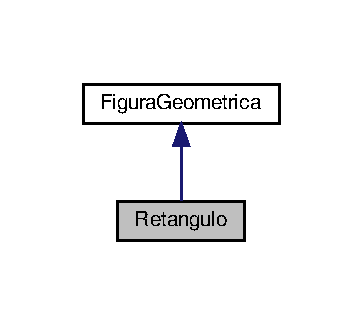
\includegraphics[width=174pt]{class_retangulo__inherit__graph}
\end{center}
\end{figure}


Collaboration diagram for Retangulo\+:
\nopagebreak
\begin{figure}[H]
\begin{center}
\leavevmode
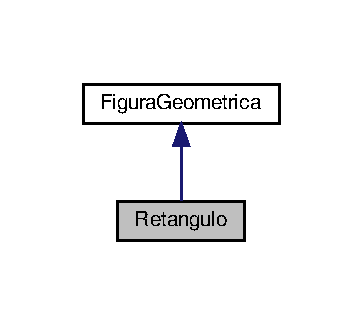
\includegraphics[width=174pt]{class_retangulo__coll__graph}
\end{center}
\end{figure}
\subsection*{Public Member Functions}
\begin{DoxyCompactItemize}
\item 
\hyperlink{class_retangulo_a3ab444178608ed5efab9889fb5780158}{Retangulo} (int x\+\_\+, int y\+\_\+, int lar\+\_\+, int alt\+\_\+, bool fill\+\_\+=false)
\begin{DoxyCompactList}\small\item\em \hyperlink{class_retangulo}{Retangulo} Cria um retângulo a partir do canto superior esquerdo e da largura e da altura. \end{DoxyCompactList}\item 
void \hyperlink{class_retangulo_ac088dd6d3f4f3d3f80363a868c2e74f1}{draw} (\hyperlink{class_screen}{Screen} \&t)
\begin{DoxyCompactList}\small\item\em draw Desenha um retângulo na tela t. \end{DoxyCompactList}\end{DoxyCompactItemize}


\subsection{Detailed Description}
The \hyperlink{class_retangulo}{Retangulo} class É uma classe concreta derivada d classe \hyperlink{class_figura_geometrica}{Figura\+Geometrica} que cria um retângulo. 

\subsection{Constructor \& Destructor Documentation}
\mbox{\Hypertarget{class_retangulo_a3ab444178608ed5efab9889fb5780158}\label{class_retangulo_a3ab444178608ed5efab9889fb5780158}} 
\index{Retangulo@{Retangulo}!Retangulo@{Retangulo}}
\index{Retangulo@{Retangulo}!Retangulo@{Retangulo}}
\subsubsection{\texorpdfstring{Retangulo()}{Retangulo()}}
{\footnotesize\ttfamily Retangulo\+::\+Retangulo (\begin{DoxyParamCaption}\item[{int}]{x\+\_\+,  }\item[{int}]{y\+\_\+,  }\item[{int}]{lar\+\_\+,  }\item[{int}]{alt\+\_\+,  }\item[{bool}]{fill\+\_\+ = {\ttfamily false} }\end{DoxyParamCaption})}



\hyperlink{class_retangulo}{Retangulo} Cria um retângulo a partir do canto superior esquerdo e da largura e da altura. 


\begin{DoxyParams}{Parameters}
{\em x\+\_\+} & É a coordenada x do canto superior esquerdo. \\
\hline
{\em y\+\_\+} & É a coordenada y do canto superior esquerdo. \\
\hline
{\em lar\+\_\+} & É a largura do retângulo. \\
\hline
{\em alt\+\_\+} & É a altura do retângulo. \\
\hline
{\em fill\+\_\+} & Determina se o retângulo será preenchido (true) ou não (false). \\
\hline
\end{DoxyParams}


\subsection{Member Function Documentation}
\mbox{\Hypertarget{class_retangulo_ac088dd6d3f4f3d3f80363a868c2e74f1}\label{class_retangulo_ac088dd6d3f4f3d3f80363a868c2e74f1}} 
\index{Retangulo@{Retangulo}!draw@{draw}}
\index{draw@{draw}!Retangulo@{Retangulo}}
\subsubsection{\texorpdfstring{draw()}{draw()}}
{\footnotesize\ttfamily void Retangulo\+::draw (\begin{DoxyParamCaption}\item[{\hyperlink{class_screen}{Screen} \&}]{t }\end{DoxyParamCaption})\hspace{0.3cm}{\ttfamily [virtual]}}



draw Desenha um retângulo na tela t. 


\begin{DoxyParams}{Parameters}
{\em t} & Tela em que será desenhada o retângulo. \\
\hline
\end{DoxyParams}


Implements \hyperlink{class_figura_geometrica_a8ee8dedc060b6059a805ea091aef2c41}{Figura\+Geometrica}.



The documentation for this class was generated from the following files\+:\begin{DoxyCompactItemize}
\item 
retangulo.\+h\item 
retangulo.\+cpp\end{DoxyCompactItemize}

\hypertarget{class_screen}{}\section{Screen Class Reference}
\label{class_screen}\index{Screen@{Screen}}


The \hyperlink{class_screen}{Screen} class funciona criando e editando telas de desenho.  




{\ttfamily \#include $<$screen.\+h$>$}

\subsection*{Public Member Functions}
\begin{DoxyCompactItemize}
\item 
\mbox{\Hypertarget{class_screen_ae7576476fc6e6a6eaa66389fdc41fe72}\label{class_screen_ae7576476fc6e6a6eaa66389fdc41fe72}} 
\hyperlink{class_screen_ae7576476fc6e6a6eaa66389fdc41fe72}{Screen} ()
\begin{DoxyCompactList}\small\item\em \hyperlink{class_screen}{Screen} Cria uma tela vazia sem tamanho e define o brush como \textquotesingle{}\#\textquotesingle{}. \end{DoxyCompactList}\item 
\hyperlink{class_screen_ab41e0f2754e0a7831a8fc3211bcdabca}{Screen} (int nlin\+\_\+, int ncol\+\_\+)
\begin{DoxyCompactList}\small\item\em \hyperlink{class_screen}{Screen} Cria uma tela vazia de tamanho pŕe-\/definido e com brush padrão \char`\"{}\#\char`\"{}. \end{DoxyCompactList}\item 
void \hyperlink{class_screen_a12eef567d26f6cb00981da6384be2eac}{new\+Matriz} (int nlin\+\_\+, int ncol\+\_\+)
\begin{DoxyCompactList}\small\item\em new\+Matriz Define o tamanho de uma tela. \end{DoxyCompactList}\item 
void \hyperlink{class_screen_ae6bea81c57a22d226507c3c26fa95ee0}{set\+Pixel} (int x, int y)
\begin{DoxyCompactList}\small\item\em set\+Pixel Desenha um pixel da matriz usando o caratere guardado em \textquotesingle{}brush\textquotesingle{} \end{DoxyCompactList}\item 
\mbox{\Hypertarget{class_screen_a35e74266b2a04e37b354ceff7a5f1031}\label{class_screen_a35e74266b2a04e37b354ceff7a5f1031}} 
void \hyperlink{class_screen_a35e74266b2a04e37b354ceff7a5f1031}{clear} ()
\begin{DoxyCompactList}\small\item\em clear Limpa a tela. \end{DoxyCompactList}\item 
void \hyperlink{class_screen_a01312ae6a1168ec0a02c24877059571f}{set\+Brush} (char brush\+\_\+)
\begin{DoxyCompactList}\small\item\em set\+Brush Muda o caractére do desenho. \end{DoxyCompactList}\end{DoxyCompactItemize}
\subsection*{Friends}
\begin{DoxyCompactItemize}
\item 
ostream \& \hyperlink{class_screen_aab6a2880746bfe1b7964817cc8f0989e}{operator$<$$<$} (ostream \&os, \hyperlink{class_screen}{Screen} \&t)
\begin{DoxyCompactList}\small\item\em operator $<$$<$ Envia um objeto da classe \hyperlink{class_screen}{Screen} como saída. \end{DoxyCompactList}\end{DoxyCompactItemize}


\subsection{Detailed Description}
The \hyperlink{class_screen}{Screen} class funciona criando e editando telas de desenho. 

\subsection{Constructor \& Destructor Documentation}
\mbox{\Hypertarget{class_screen_ab41e0f2754e0a7831a8fc3211bcdabca}\label{class_screen_ab41e0f2754e0a7831a8fc3211bcdabca}} 
\index{Screen@{Screen}!Screen@{Screen}}
\index{Screen@{Screen}!Screen@{Screen}}
\subsubsection{\texorpdfstring{Screen()}{Screen()}}
{\footnotesize\ttfamily Screen\+::\+Screen (\begin{DoxyParamCaption}\item[{int}]{nlin\+\_\+,  }\item[{int}]{ncol\+\_\+ }\end{DoxyParamCaption})}



\hyperlink{class_screen}{Screen} Cria uma tela vazia de tamanho pŕe-\/definido e com brush padrão \char`\"{}\#\char`\"{}. 


\begin{DoxyParams}{Parameters}
{\em nlin\+\_\+} & Número de linhas da matriz da tela \\
\hline
{\em ncol\+\_\+} & Número de colunas da matriz da tela \\
\hline
\end{DoxyParams}


\subsection{Member Function Documentation}
\mbox{\Hypertarget{class_screen_a12eef567d26f6cb00981da6384be2eac}\label{class_screen_a12eef567d26f6cb00981da6384be2eac}} 
\index{Screen@{Screen}!new\+Matriz@{new\+Matriz}}
\index{new\+Matriz@{new\+Matriz}!Screen@{Screen}}
\subsubsection{\texorpdfstring{new\+Matriz()}{newMatriz()}}
{\footnotesize\ttfamily void Screen\+::new\+Matriz (\begin{DoxyParamCaption}\item[{int}]{nlin\+\_\+,  }\item[{int}]{ncol\+\_\+ }\end{DoxyParamCaption})}



new\+Matriz Define o tamanho de uma tela. 


\begin{DoxyParams}{Parameters}
{\em Número} & de linhas da matriz da tela \\
\hline
{\em ncol\+\_\+} & Número de colunas da matriz da tela \\
\hline
\end{DoxyParams}
\mbox{\Hypertarget{class_screen_a01312ae6a1168ec0a02c24877059571f}\label{class_screen_a01312ae6a1168ec0a02c24877059571f}} 
\index{Screen@{Screen}!set\+Brush@{set\+Brush}}
\index{set\+Brush@{set\+Brush}!Screen@{Screen}}
\subsubsection{\texorpdfstring{set\+Brush()}{setBrush()}}
{\footnotesize\ttfamily void Screen\+::set\+Brush (\begin{DoxyParamCaption}\item[{char}]{brush\+\_\+ }\end{DoxyParamCaption})}



set\+Brush Muda o caractére do desenho. 


\begin{DoxyParams}{Parameters}
{\em brush\+\_\+} & Carcatére o desenho. \\
\hline
\end{DoxyParams}
\mbox{\Hypertarget{class_screen_ae6bea81c57a22d226507c3c26fa95ee0}\label{class_screen_ae6bea81c57a22d226507c3c26fa95ee0}} 
\index{Screen@{Screen}!set\+Pixel@{set\+Pixel}}
\index{set\+Pixel@{set\+Pixel}!Screen@{Screen}}
\subsubsection{\texorpdfstring{set\+Pixel()}{setPixel()}}
{\footnotesize\ttfamily void Screen\+::set\+Pixel (\begin{DoxyParamCaption}\item[{int}]{x,  }\item[{int}]{y }\end{DoxyParamCaption})}



set\+Pixel Desenha um pixel da matriz usando o caratere guardado em \textquotesingle{}brush\textquotesingle{} 


\begin{DoxyParams}{Parameters}
{\em x} & É a coordenada \textquotesingle{}x\textquotesingle{} do pixel a ser inserido. \\
\hline
{\em y} & É a coordenada \textquotesingle{}x\textquotesingle{} do pixel a ser inserido. \\
\hline
\end{DoxyParams}


\subsection{Friends And Related Function Documentation}
\mbox{\Hypertarget{class_screen_aab6a2880746bfe1b7964817cc8f0989e}\label{class_screen_aab6a2880746bfe1b7964817cc8f0989e}} 
\index{Screen@{Screen}!operator$<$$<$@{operator$<$$<$}}
\index{operator$<$$<$@{operator$<$$<$}!Screen@{Screen}}
\subsubsection{\texorpdfstring{operator$<$$<$}{operator<<}}
{\footnotesize\ttfamily ostream\& operator$<$$<$ (\begin{DoxyParamCaption}\item[{ostream \&}]{os,  }\item[{\hyperlink{class_screen}{Screen} \&}]{t }\end{DoxyParamCaption})\hspace{0.3cm}{\ttfamily [friend]}}



operator $<$$<$ Envia um objeto da classe \hyperlink{class_screen}{Screen} como saída. 


\begin{DoxyParams}{Parameters}
{\em os} & Função de saída da biblioteca padrão c++ \\
\hline
{\em t} & Objeto que será impresso. \\
\hline
\end{DoxyParams}
\begin{DoxyReturn}{Returns}
Impressão do objeto t. 
\end{DoxyReturn}


The documentation for this class was generated from the following files\+:\begin{DoxyCompactItemize}
\item 
screen.\+h\item 
screen.\+cpp\end{DoxyCompactItemize}

%--- End generated contents ---

% Index
\backmatter
\newpage
\phantomsection
\clearemptydoublepage
\addcontentsline{toc}{chapter}{Index}
\printindex

\end{document}
